\chapter{Paraphotons}
\label{chap:Paraphotons}

\section{Theory and Motivation}
	The standard model of particle physics is a testament to the power of theory in modern particle physics. However, there are some topics that require additional physics, for example, it has no explanation for dark matter or dark energy and assumes a zero-mass neutrino.  There are some known extensions to the standard model that introduce new physics capable of explaining both at the same time. Many of these theories require  a new, hidden sector of particles which only interact with the standard, visible sector of particles via forces with very weak couplings. Under one possible version of a hidden sector theory, in addition to the well-known photon there exists a paraphoton ($\gamma \prime$ ) with finite mass. A simple Lagrangian for this case has been developed by Afanasev \cite{Para_Afanasev} of the form shown in eqn. \ref{Lagrangian}
	\begin{equation}
	\mathcal{L} = -\frac{1}{4}F^{\mu\nu}F_{\mu\nu} - \frac{1}{4}B^{\mu\nu}B_{\mu\nu} -\frac{1}{2} \chi F^{\mu\nu}B_{\mu \nu} + \frac{1}{2} m_{\gamma'}^2 B_\mu B^\mu
	\label{Lagrangian}
	\end{equation}
	 In eqn. \ref{Lagrangian} \emph{F} is the electromagnetic gauge field strength tensor, \emph{B} is the field strength tensor for the hidden sector, $\chi$ is the mixing parameter between photons and paraphotons and $m_{\gamma'}$ is the paraphoton mass. Motivations and constraints  for a Lagrangian of this form come primarily from anomalous results from the AMS and EGRET experiments \cite{Para_Justification}. The PAMELA experiment detected an unexpected positron excess between 10 and 100 GeV \cite{PAMELA}, which was later confirmed and expanded upon by the AMS experiment \cite{AMS}.  A graph of the AMS positron excess can be seen in Fig. \ref{Pam_Graph}. 

\begin{figure}
\caption{A comparison of AMS results with other recent published measurements.}
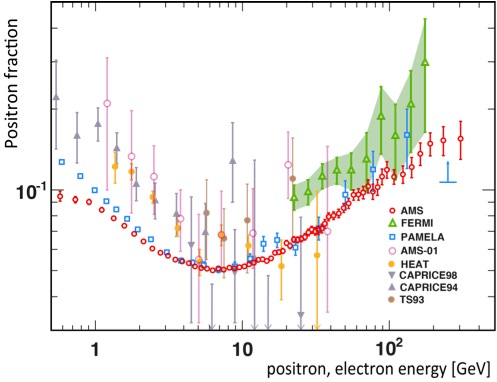
\includegraphics[width=\textwidth]{Paraphotons/AMS_Positron.jpg}
\label{Pam_Graph}
\end{figure}

This excess can best be explained by a dark matter annihilation into $e^+ e^-$ pairs, but this requires a very large annihilation cross-section.  The annihilation cross-section required is much larger than what is allowed by thermal relic abundance. Additionally, thermal dark matter particles would require boost factors of $O(100)$ or more above expectation to explain the AMS excesses. The AMS results also require simultaneously a high cross-section for lepton production and a low cross-section for hadron production. 

Generating sufficiently high energy electrons and positrons is generally associated with $W^{\pm}$ and $Z^{0}$ boson decay, as they produce equal amounts of electrons and positrons, and give both particles a large amount of energy. However, the high energy electrons and positrons required are not a good match to $Z^{0}$ or $W^{\pm}$ boson decays , as $Z^{0}$'s  produce very few hard leptons and while $W$'s can produce the required high energy leptons, they also produce copious amounts softer leptons, which are not seen in the AMS data. 

Similarly, the EGRET experiment  observed a larger than expected $\gamma$ flux between 10 and 50 GeV \cite{EGRET}. This excess could be explained through inverse-Compton scattering of high energy electrons and positrons off of Cosmic Microwave Background radiation. Although the high energy excess was not confirmed by the newer Fermi-LAT probe, the results from Fermi-LAT do not rule out a contribution from dark matter annihilation. 


\begin{figure}
\caption{EGRET re-analysis by Strong \emph{et} \emph{al.} \cite{EG_Strong} showing a break in the trend for $E > 2 \times 10^4$ keV.}
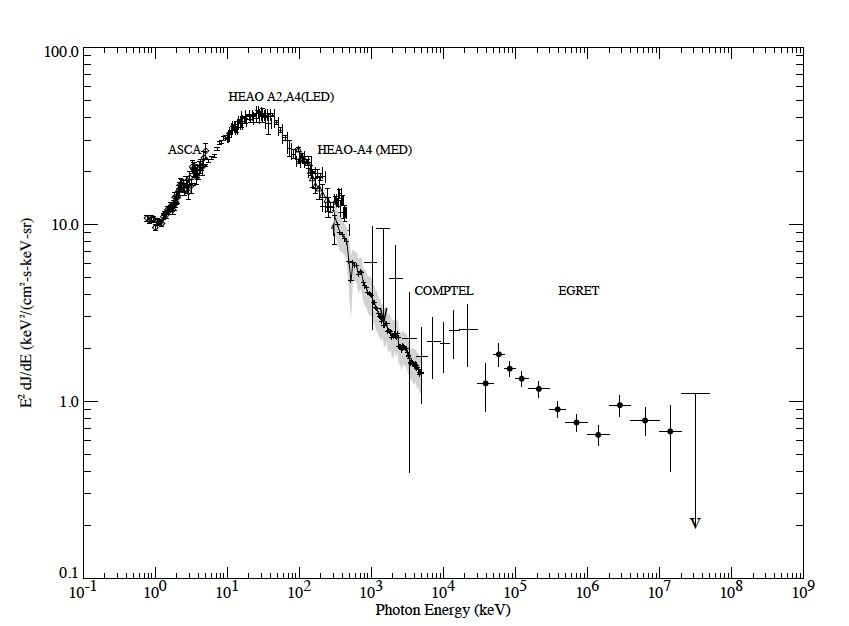
\includegraphics[width=\textwidth]{Paraphotons/EGRET.jpg}
\label{EG_Graph}
\end{figure}

The results suggest a dark matter particle which is charged under a new U(1) hypercharge. One such model is a Chameleon Vector Boson Model \cite{Camo_Vector}, which predicts a paraphoton: a light electrically neutral particle with a U(1) hypercharge corresponding to a conserved baryon number -lepton number (B-L). This model also explains relatively small neutrino masses \cite{Vector_Boson}. 

 \section{Prior Searches}
  There have been previous attempts to detect paraphotons, generally in the context of axion and other hidden sector particle searches. The primary experimental method used is the ``Light Shining Through a Wall" (LSW) technique. This involves shining a beam of photons of a particular wavelength at a ``wall:" a material that is impenetrable to the photons. Some of the light will oscillate into paraphotons before it strikes the wall, and pass through the wall without being absorbed. After passing through the wall, the paraphotons can oscillate back into photons, yielding a detectable signal.  Experiments which utilize this technique include GammeV \cite{GammeV}, BMV \cite{BMV}, OSQAR \cite{OSQAR}, and, more recently, SPring-8 \cite{2013PhLB..722..301I}. 
  
  Other experiments have used microwave cavities \cite{Parker:2013fba} for paraphoton searches. This group of experiments uses a standing microwave established in one cavity, while a second spatially separated cavity is monitored. Using the same principles as the LSW experiments, a photon in one cavity has a probability of transforming into a paraphoton, moving through barriers, and then oscillating back to a photon inside the second cavity.  Similarly, a photon in the second cavity has the same ability to move from the second cavity back to the first, using the same $ \gamma \rightarrow \gamma \prime \rightarrow \gamma$ reaction. Thus, paraphotons cause coupling between the two cavities in a fashion similar to a pair of coupled oscillators. Further details of this method is beyond the scope of this thesis, but can be seen in the Parker paper \cite{Parker:2013fba}. The established limits on paraphoton parameters, as of the SPring-8 results, can be seen in Fig. \ref{Limits}.
 
 \begin{figure}
 \caption{SPring-8 limits on paraphoton mass and photon/paraphoton mixing parameter ($\chi$)  \cite{2013PhLB..722..301I}.}
 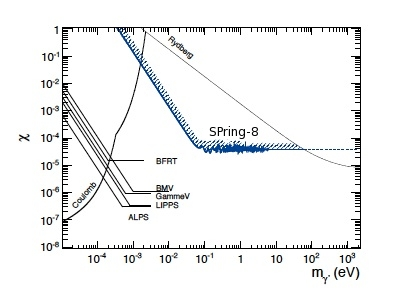
\includegraphics[width=.5 \textwidth]{Paraphotons/Spring_Limits_edit.jpg}
 \label{Limits}
 \end{figure}


\section{Analysis Overview}
The Double Chooz experiment is very well suited to detect paraphotons, with a powerful, well-calibrated source of $\gamma$s in the form of the Chooz B1 and B2 reactors. If these $\gamma$s can oscillate into paraphotons, some will decay inside of the Double Chooz target volume, producing a detectable signal. In a sense, the Double Chooz experiment works as an extension of the ``LSW" method. Our search has two primary advantages over prior searches: a (comparatively) large target volume and a (comparatively) intense source of initial photons. Because of these advantages, we are capable of probing areas of the (mass, mixing)-space which have been inaccessible to prior searches. However, there are a number of challenges to extracting a clean signal. 

We will begin by discussing the expected signal and our sensitivity to paraphotons. We will then follow the chain of analysis, beginning with simulation, and proceeding through background fitting and, finally, signal fitting. We will then discuss the results of our search, and the opportunities presented by the Double Chooz Near Detector, which is scheduled to come online in 2014-2015. 

\section{Expected Signal}
The total expected signal as a function of energy is expressed by Eq. \ref{Npara}: 

\begin{equation}
N_{det}(E) = N_{\gamma}(E) F_{Ar}(E) F_{De}(E)  \frac{1}{4 \pi}  \Omega R_{Branch} (\chi)^2 \epsilon(E)
\label{Npara}
\end{equation}

This section will discuss each of the terms in turn, save for $\epsilon $, the detection efficiency, which will be discussed in Sec \ref{sec:Cuts}.  We will, for purposes of this calculation, examine only the Double Chooz Far Detector. Considerations of the Double Chooz Near Detector will be handled in Sec. \ref{sec:Future_Work}.

We begin with $N_{\gamma}$, the number of $\gamma$s produced by the reactors. The vast majority are prompt $\gamma$s produced from fission products, but there are non-trivial contributions from $\beta$-decay products, nuclear de-excitation of reactor moderators and fuel rods, and from ineleastic nuclear scattering. From studies of the Julich research reactor \cite{Chris_Jones}, the contributions of these sources give a parameterized total photon rate, $N_{\gamma}$ of the form: $N_{\gamma}(E) = e^{-E_{\gamma}/0.91 [MeV]} \cdot (0.58 \times 10^{18} /MW /s) \cdot P_{th}  $, where $P_{th}$ is the thermal power of the reactor and $E$ is the energy of the $\gamma$. This expression is valid for $\gamma$ energies above 1 MeV. The spectrum is shown in Fig. \ref{Gamma_Flux}.

\begin{figure}
\caption{Predicted Double Chooz reactor $\gamma$ spectrum for energy $>$ 1 MeV showing the large expected $\gamma$ production ($>10^{18}$).}
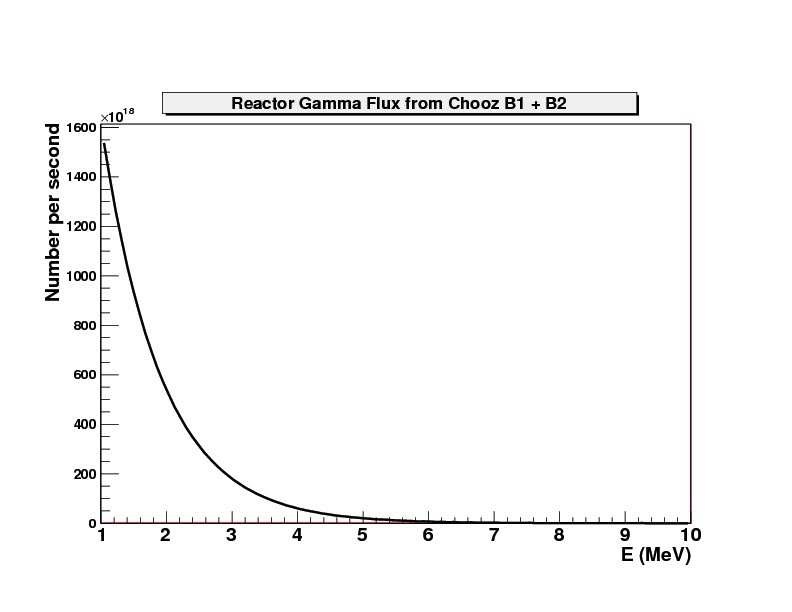
\includegraphics[width=\textwidth]{Paraphotons/Gamma_Flux.jpg}
\label{Gamma_Flux}
\end{figure}
 
The next two terms, $F_{Ar}(E)$ and $F_{De}(E)$ are the fraction of arriving and decaying paraphotons, respectively.  The decay length of a paraphoton of mass $M_{Para}$ is given by $D_{Para} = \gamma c \tau_{Para} = \frac{E_{Para}}{M_{Para}}$. The probability of survival for a given decay length ($D_{Para}$) and distance to the target ($D_{target}$) is thus $e^{-(D_{target}/D_{Para})}$. Since the detector is 1 kilometer away, the fraction of arriving paraphotons is given by $F_{Ar} = e^{-1000 m /D_{Para}}$. We do not have to take into account shielding of either the reactor or the detector, as paraphotons should not be affected. Once the paraphotons arrive, they must decay inside the 2.3 meter diameter detector to be detected, so $F_{De} = 1- e^{-2.3 m /D_{Para}}$.

The next two terms handle geometrical effects. The first, $\frac{1}{4 \pi}$, takes the raw rate of $\gamma$s generated at the reactors and spreads it over $4 \pi$ of solid angle. The next term, $\Omega$ handles the solid angle subtended by the detector. The Double Chooz target has a height of 2.46 meters and a radius of 1.15 meters and is cylindrical in shape \cite{DC_2012}, giving a cross section of 5.66 m$^2$, which translates to a solid angle of $\frac{5.66}{r^2}$ where $r$ is the distance from the reactor cores to the detector. 

The next two terms are model dependent. The term $R_{Branch}$ is the branching ratio to a detectable signal. The paraphoton is predicted to have  primary decay mode of $\gamma \prime \rightarrow \nu \bar{\nu}$, which  is not detectable by our analysis. The paraphoton may also decay into 3 or 5 $\gamma$s ( $\gamma \prime \rightarrow 3 \gamma$ or $\gamma \prime \rightarrow 5 \gamma$).  Of these two, the 3 $\gamma$ case is strongly favored. Our model uses a branching ratio of $R_{Branch} = 10^{-7}$,  motivated by astrophysical limits \cite{Chris_Jones}. The last term addressed here is $\chi$, the oscillation parameter.  The number of $\gamma$s which oscillate into paraphotons is mass and energy independent, determined solely by the the dimensionless mixing parameter referred to in the literature as $\chi$.  


\section{Simulation}
To properly simulate paraphotons within DCGLG4sim, the official Double Chooz GEANT4 particle simulation environment, we developed a new generator for the particles. The generator begins by creating a spectrum of possible paraphoton energies, dependent on the reactor thermal power, distance to the reactor cores, and on the paraphoton mass. This spectrum is used as a probability distribution function in energy, from which an energy is selected for each paraphoton. That energy is then split between three daughter $\gamma$s inside the detector. In order to ensure that the splitting of energy follows Fermi's Golden Rule, we make use of a powerful geometrical tool. Specifically, we create a sphere of radius $R = \sqrt{E}$, where $E$ is the energy of the paraphoton. We then generate a point on the surface of the sphere, which describes the $X$, $Y$ and $Z$ co-ordinate of the point corresponding to the energies of the three daughter particles as per $\sqrt{E_1^2 + E_2^2 + E_3^2}  = E$. We impose a further condition that no one $\gamma$ has more energy than the other two combined, as such a situation would result in a non-conservation of momentum. We then use the same technique to divide up momentum between the three particles to ensure that momentum is conserved. 

The paraphoton decay signals have been produced in the Monte Carlo and used to generate events which are run through the standard analysis chain, simulating the effect of detector readout and pulse, position, and energy  reconstruction. These signals can then be mixed with  data or similarly processed Monte Carlo signals to allow for fine tuning of cuts, validation of the analysis chain, and backgrounds. 


\section{Analysis and Data Processing}
\subsection{Analysis Overview}
  Now that we have a simulated sample of paraphoton events, we can begin to search the Double Chooz dataset for a similar signal. We begin by developing a set of cuts which are used to remove or reduce unwanted background events. Once these cuts have been developed, we use them on a sample of pure background data to develop a model of backgrounds which can be scaled up to the larger data sample which may contain paraphoton events. We also inject a set of simulated paraphoton decays into a sample of pure background data, and attempt to reconstruct the signal to validate the analysis technique. After that, we perform this analysis on the full Double Chooz 3rd publication dataset and attempt to find a paraphoton signal.

\subsection{Cuts}
\label{sec:Cuts}
Because the number of background events dwarfs the number of expected paraphoton events, it is vital to develop a set of cuts to improve the ratio of expected paraphoton events to background. The cuts used are very similar to those used by Double Chooz in the search for neutrinos, but there are unique refinements designed to select for paraphotons decays rather than neutrino events. 
	
  We begin by filtering out cosmic ray muon events from the sample, making use of the official Double Chooz muon cuts. These cuts make use of the Inner Veto (IV) , but not the Outer Veto (OV), as OV data is not available for all runs in the dataset. We make the following cuts to identify muons: more than 200 MeV of energy deposited in the Neutrino Target (NT) or more than 30,000 DUQ (digital units of charge, approximately 15000 DUQ is 1 MeV) in the IV. The use of DUQ in the inner detector is because the exact relationship between DUQ and energy in the inner detector is not as well calibrated as the relationship in the NT. A graph of the muon cuts plotted against a reference Double Chooz singles spectrum from the 3rd publication can be seen in Fig. \ref{Muon_Cuts}. 
  
  \begin{figure}
  \caption{IV (top) and ID (bottom) charge distribution in Double Chooz singles. Muon cuts are marked in red.}
  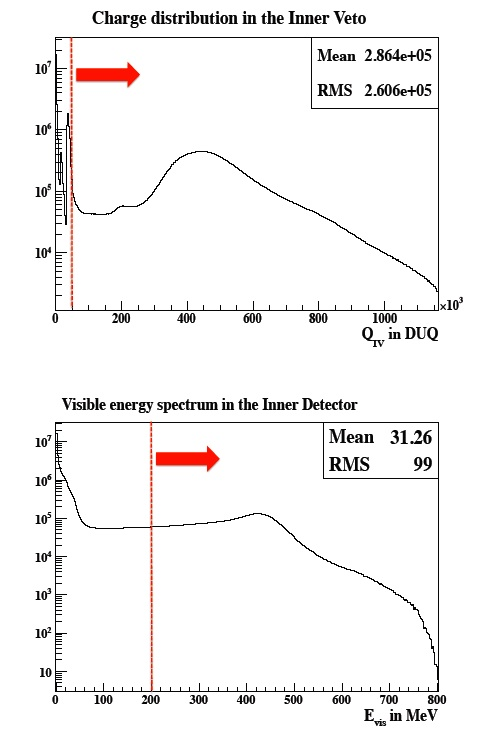
\includegraphics[height=.9 \textheight]{Paraphotons/Muon_Cuts.jpg}
  \label{Muon_Cuts}
  \end{figure}

After we identify muon-like signals, we implement a post-muon cut of 1 millisecond to reduce the contribution of cosmogenic muon products to the signal. These isotopes are produced by muon interactions with $^{12}$C, either spallation or muon capture. In both cases, relatively long lived but unstable isotopes, such as $^{9}$B, $^{9}$Li, $^{10}$C, or $^{11}$C. Unfortunately, most of the cosmogenics of interest, particularly $^{12}$C, $^{12}$B, and $^{11}$C, are not eliminated by this cut, but their contribution to the signal is reduced. 

After the post-muon cut, there is a set of ``light noise" cuts, designed to eliminate PMT-based backgrounds. There are three parts to light noise elimination. First, an ``MQTQ" cut, which compares the maximum charge on any PMT with the total charge in the event, as light noise events tend to have signals localized to a single PMT. Second, a ``Qdiff" cut eliminates events which have a very large difference in charge seen between the PMT with the largest charge and surrounding PMTs, as a physical event will tend to deposit similar amounts of charge on nearby PMTs. Finally, there is a ``two-part" cut, which cuts on a combination of the RMS of the charge and the RMS of the start time of the event on each PMT. A graph of this last cut can be seen in Fig. \ref{LightNoise}.

\begin{figure}
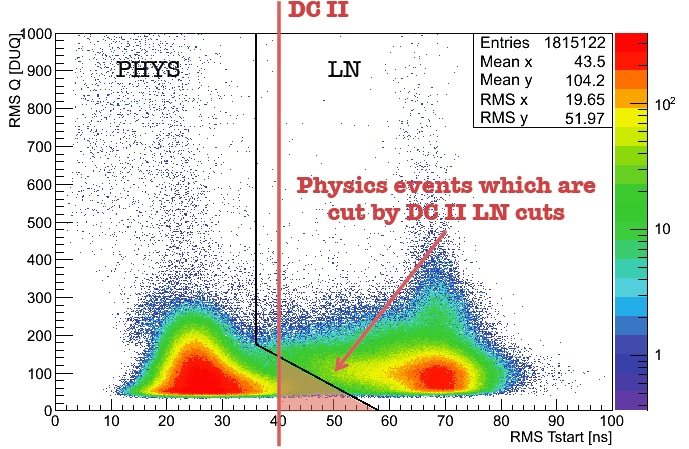
\includegraphics[width=\textwidth]{Paraphotons/Light_Noise_Cuts.jpg}
\caption{Light noise cuts in this work (in black) vs. those used in the DC 2nd publication (in red).}
\label{LightNoise}
\end{figure}

The specific value for the cuts used are as follows: $MQTQ< 0.12$, $Q_{Diff} < 30000$ DUQ, and $RMS_{Tstart} < 36 $ns  or $RMS_{Q} < 464- 8 \times RMS_{Tstart}$ for the ``two-part" cut. Events which do not have values in this range are discarded. These cuts are the same as are used for the Double Chooz 3rd publication \cite{DC_2014}, and have been extensively validated. Simulated paraphoton events are not removed by these cuts, but the presence of light noise in the signal is sharply reduced. 

In order to reduce the background from radioactive isotopes in the rock and target vessel, we made use of a position isolation cut, considering only events which fall in the inner part of the NT. This cut requires $\rho <100 $cm and $Z < \pm 100$ cm . This cut was used as part of the Double Chooz single studies currently ongoing, and has been validated by our collaborators \cite{Mariano}.

 To distinguish the paraphoton signal from potential backgrounds, we make use of the Double Chooz position-reconstruction algorithm, RecoBAMA. We have discussed the two-part method by which RecoBAMA reconstructs the positions of events inside of the detector in Sec. \ref{sec:RECO} of chapter 2. The first is a charge-based or ``Q" reconstruction, which, to first order, assumes that the charge from an event is spread across the surface of a sphere. Therefore, the charge seen by a PMT should vary with distance in a $\frac{1}{r^2}$ fashion, with closer PMTs seeing more light. The second reconstruction tool is a time-based, or ``T" reconstruction, which assumes that closer PMTs will see the light sooner than further PMTs. This reconstruction algorithm effectively ``blows bubbles" from PMTs that see light, and looks for an intersection point. More discussion of the exact process used can be seen Chapter \ref{chap:Double Chooz}.
 
The two reconstruction tools are used in combination for neutrino detection in Double Chooz, but for the purposes of isolating paraphoton events, the time-based reconstruction tool has the ability to help distinguish between simulated three $\gamma$ paraphoton decay events and the background events. We expected that the 3-$\gamma$ paraphoton decay events would be poorly reconstructed relative to backgrounds, as a 3-$\gamma$ event would be less able to be reconstructed to a single vertex. The ability to distinguish one from the other is not perfect, as the scintillator in the detector emits isotropically and causes the light from the paraphotons out into a more-or-less spherical shape. A graph of paraphoton signals in comparison to some common singles can be see in Fig. \ref{ParaVMC}.

\begin{figure}
\caption{Paraphotons and cosmogenic singles comparison of time-like goodness of fit and reconstructed charge.}
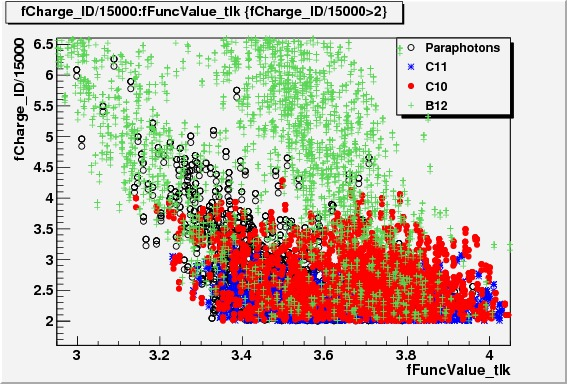
\includegraphics[width=\textwidth]{Paraphotons/ParaphotonsVMC.jpg}
\label{ParaVMC}
\end{figure}

The backgrounds in the plot are $^{12}$B, $^{11}$C, and $^{10}$C, which are the primary backgrounds in the energy range of interest. Cosmogenics are particularly troublesome, as there are very few sources of naturally occurring radiation above 2.8 MeV, and the $(n,\gamma)$ Gd capture has a well defined energy peak. The spectrum of singles events in Double Chooz can be seen in Fig. \ref{DC_Singles}.

\begin{figure}
\caption{Double Chooz singles Monte Carlo vs. measured rates. Note the Monte Carlo matches the predicted spectrum very well \cite{Lindley}. The Y axis is rate in arbitrary units.}
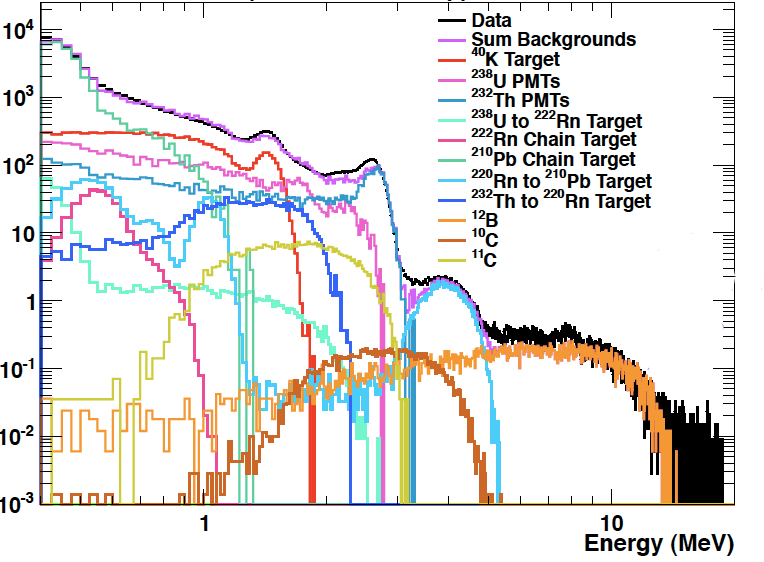
\includegraphics[width=\textwidth]{Paraphotons/Lindley_Spectrum.jpg}
\label{DC_Singles}
\end{figure}
  
It is clear that the paraphoton signal is difficult to distinguish from cosmogenic backgrounds even making use of the likelihood cuts. However, complete isolation is not required, as the paraphoton contribution to the Double Chooz energy spectrum can be analyzed by using the two-reactor-off (Off/Off) dataset to identify and model cosmogenic and radioactive backgrounds.

If the paraphotons are produced from the reactors, the Off/Off data sample should have no paraphoton events. If we model the backgrounds in the Off/Off data, we can apply that model to the two-reactor-on (On/On) data, allowing for the isolation of events which are unique to the On/On data sample. The events found only in the On/On data would be paraphotons (or other axion-like particles) and neutrinos.  Moreover, since neutrino events have a set of well-described energy features, it is possible to reduce their impact by selecting a region for analysis which lies in the ``gap" between the hydrogen and gadolinium neutron capture peaks. 


\subsection{Data Processing}
\label{sec:Data Processing}

Our analysis begins by applying the cuts described above to three data samples: the paraphoton Monte Carlo generated through DCGLG4sim and processed through the Common Trunk, the Off/Off data, and the Double Chooz 3rd publication dataset of On/On data. The data sample consists of approximately 5 days of Off/Off livetime and 156 days of On/On livetime. The paraphoton Monte Carlo sample used has approximately 20000 events, generated from paraphoton spectra corresponding to masses between 1 and 100 keV. Some samples of the paraphoton spectra used can be seen in  Fig. \ref{Para_Spec} while the approximate number of events per day can be seen in Fig. \ref{Para_Rates}.

\begin{figure}
\caption{Sample paraphoton spectra for Far Detector, at full reactor power, with various paraphoton masses.}
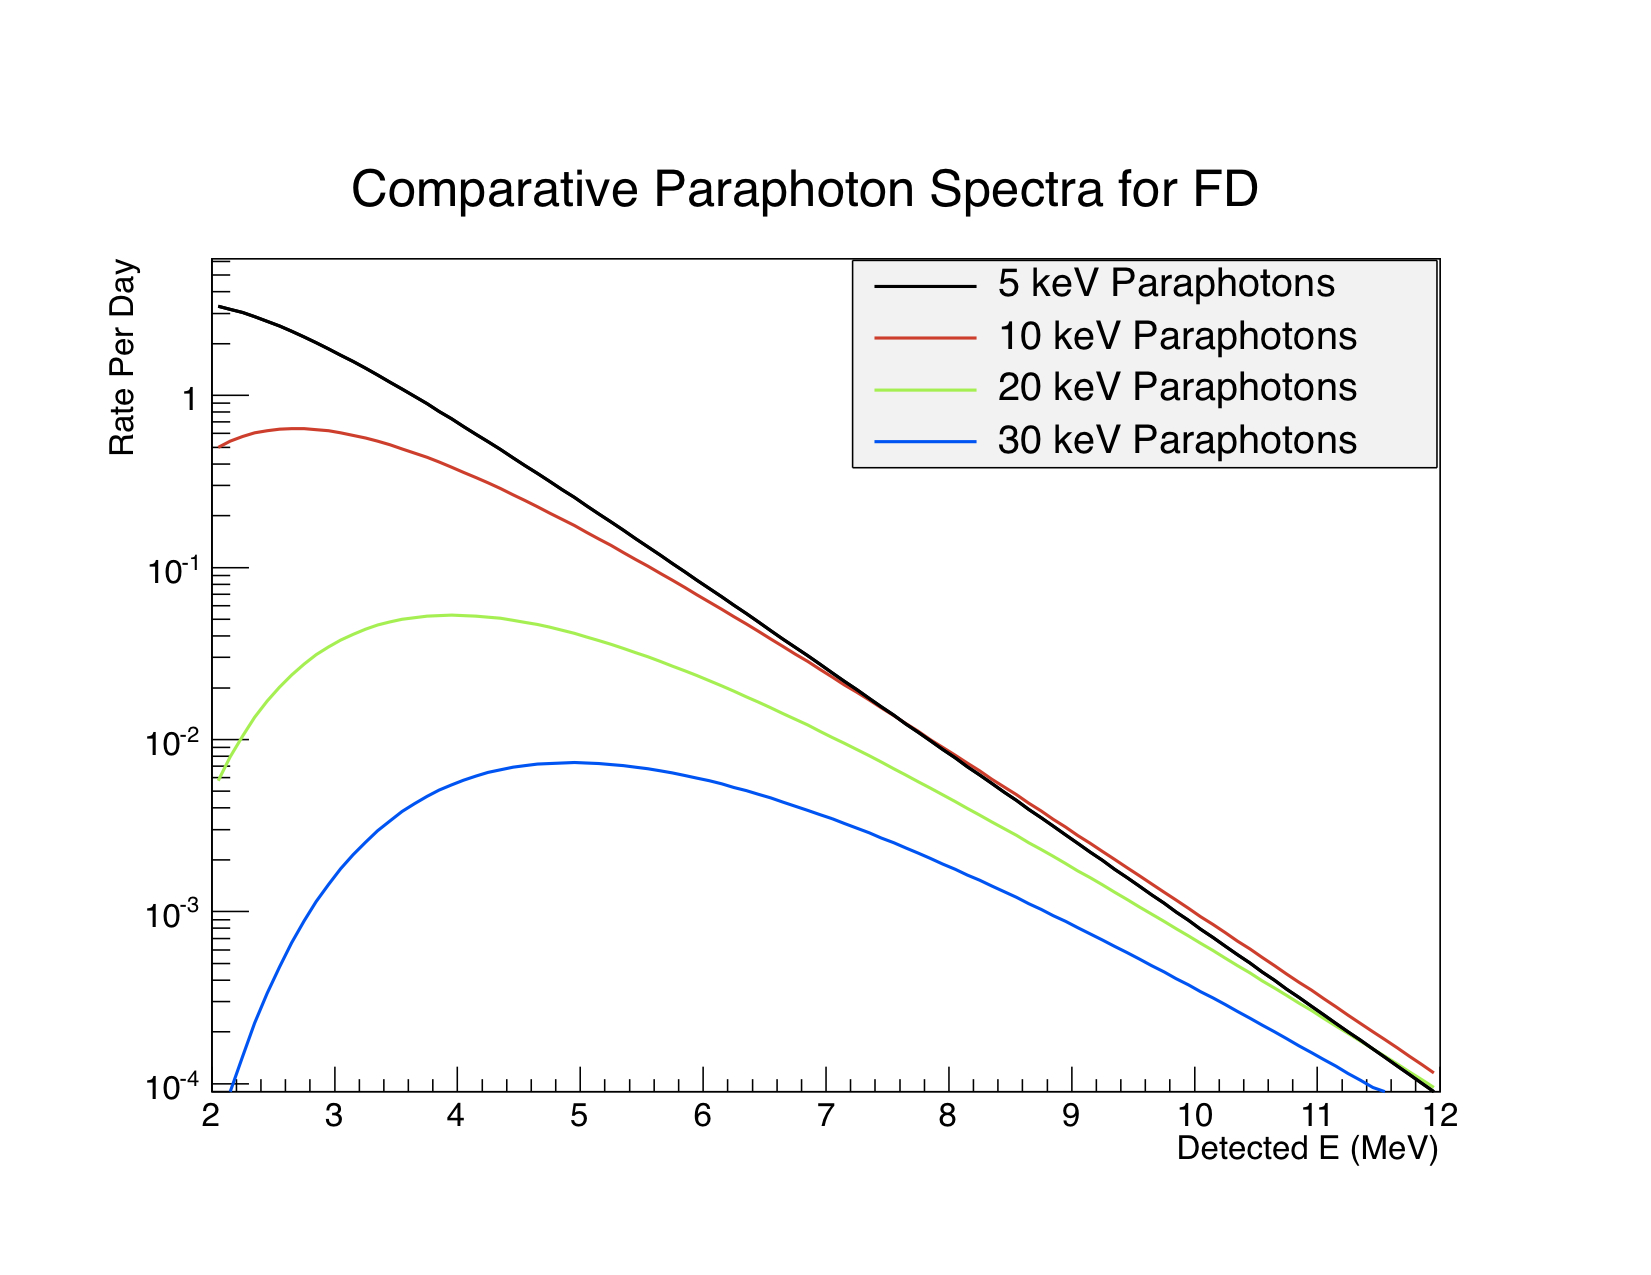
\includegraphics[width=\textwidth]{Paraphotons/Far_Theory_Spectrum.jpg}
\label{Para_Spec}
\end{figure}

\begin{figure}
\caption{Expected paraphotons detection rate per day for the Far Detector.}
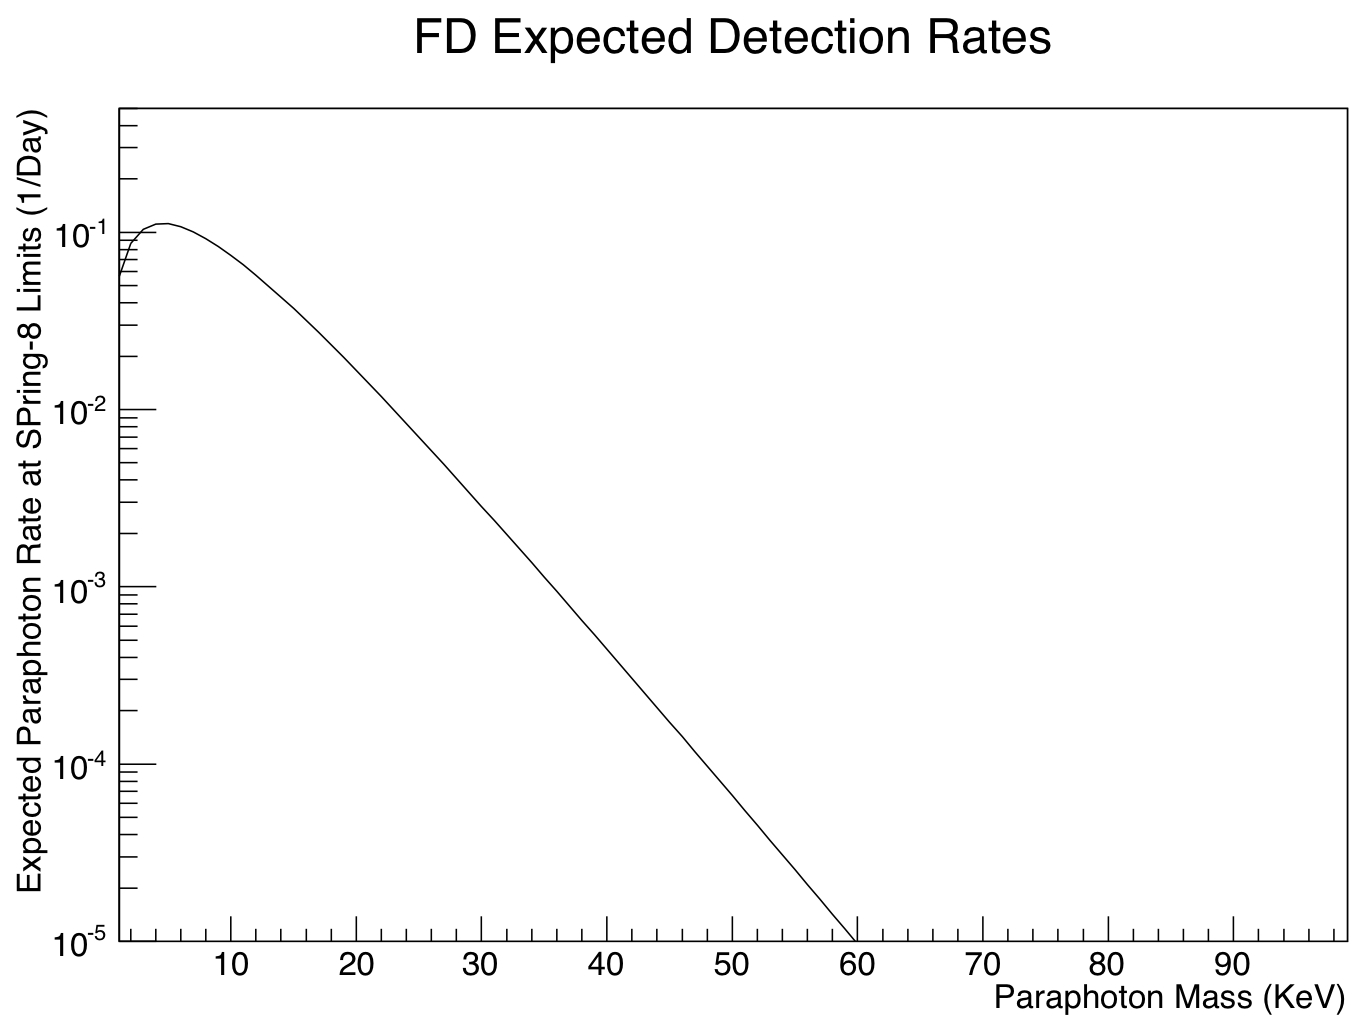
\includegraphics[width=\textwidth]{Paraphotons/FD_Expected_Detection_Rates.jpg}
\label{Para_Rates}
\end{figure}


\subsection{Off/Off Data Analysis}
  We attempted to fit a set of known background spectra to the Off-Off data sample to validate our background model. The background spectra were Monte Carlo spectra generated for the Double Chooz 3rd publication. We did not attempt to fit below 2 MeV, as backgrounds in that region are large, not well characterized, and do not affect the region of interest for our study. Our goal was to characterize the backgrounds present inside of the window between the gadolinium capture peak (centered around 8 MeV) and neutron capture on hydrogen energy peak (centered at 2.2 MeV).
  
  The primary spectra we used to fit were the cosmogenic isotopes $^{12}$B, $^{10}$C, and $^{11}$C as well as natural $^{40}$K, $^{210}$Tl and portions of the $^{220}$Ra and $^{238}$U decay chain. We found a great deal of radioactivity correlated with the Target acrylic vessel, validating our use of the target isolation cut. A picture of the Off/Off spectrum, post-cuts fit with the Mote Carlo backgrounds near of the region of interest can be seen in Fig. \ref{Off Off Fit}.
  
  \begin{figure}
\caption{ Off/Off Spectrum fit with combined Monte Carlo-produced backgrounds. This fit is not directly compared to the On/On data but is used to ensure that we understand the large features of the Off/Off dataset.}
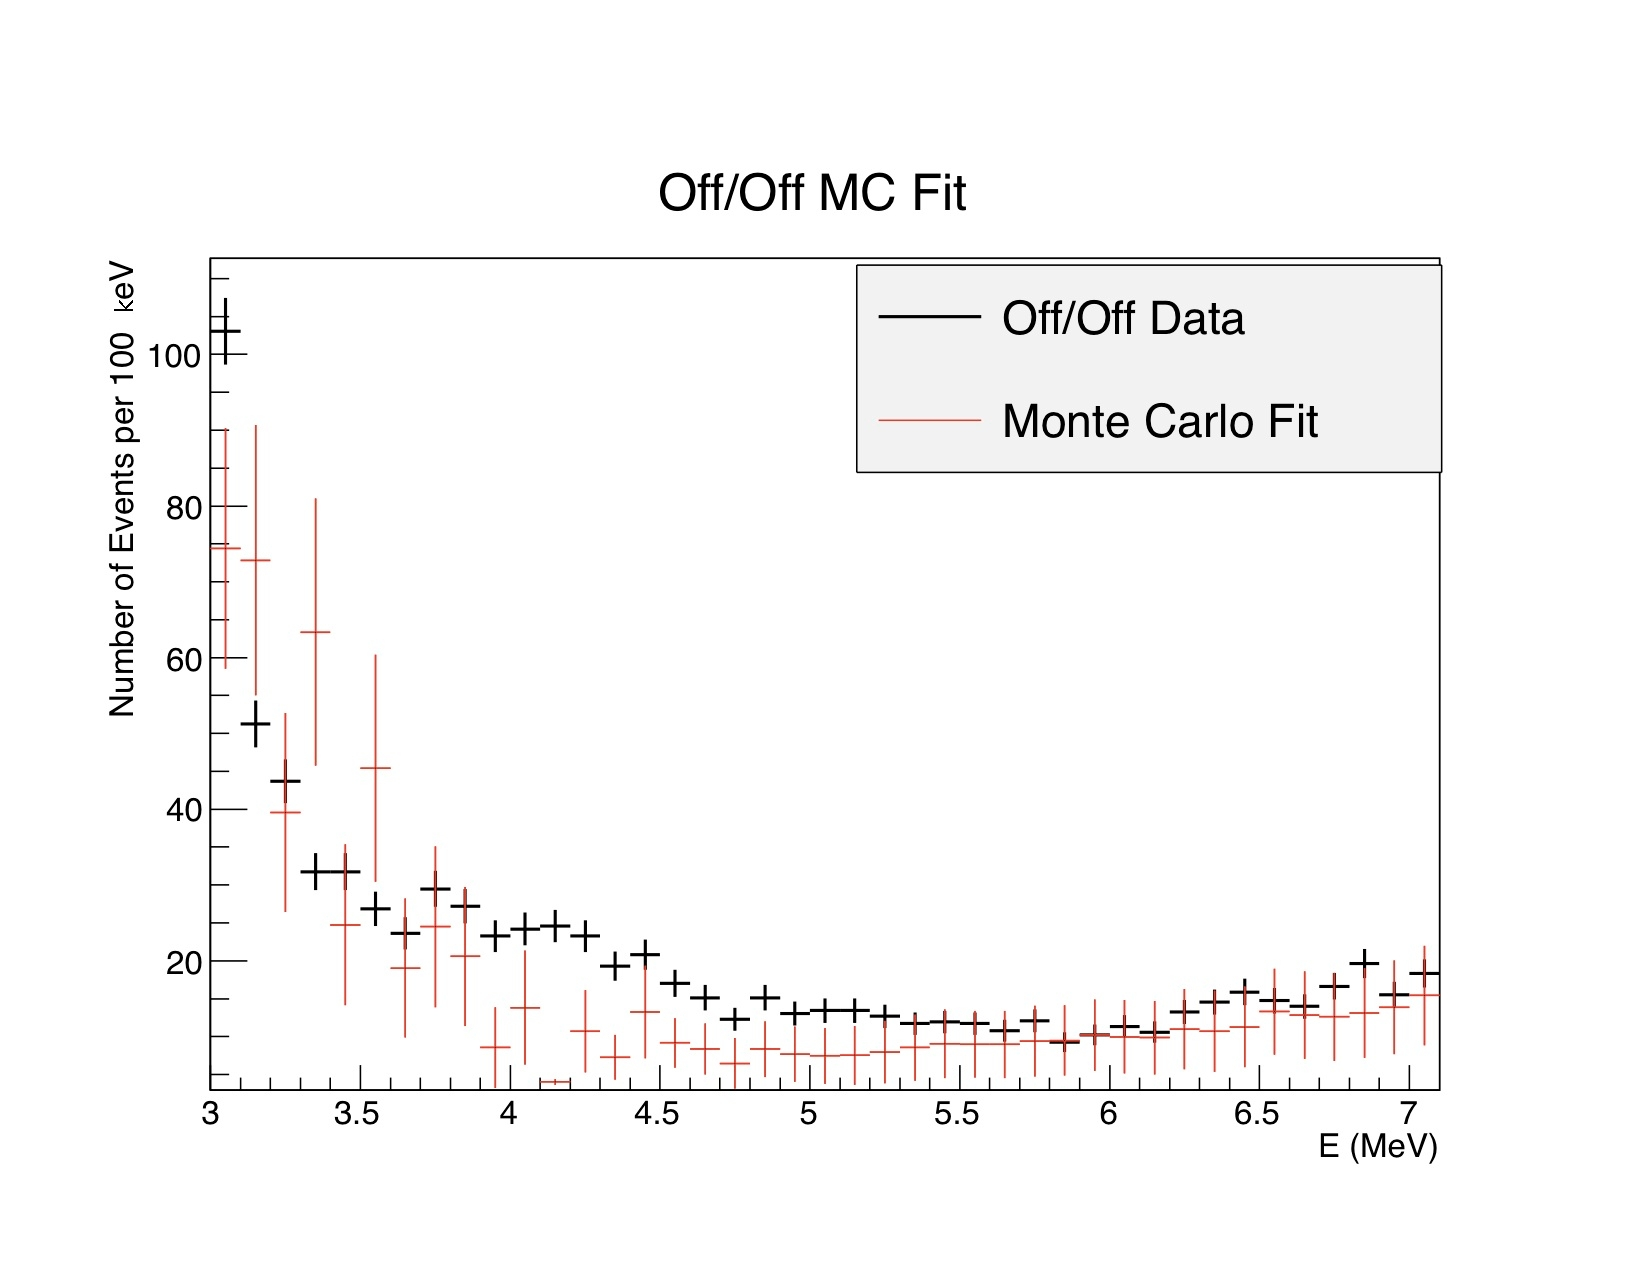
\includegraphics[width=\textwidth]{Paraphotons/OffOffMCFit_edit.jpg}
\label{Off Off Fit}
\end{figure}

Also as part of the Off/Off nalysis, we determined the exact energy region of interest for the paraphoton search. This was done by taking the ratio of the total number of Monte Carlo-produced paraphoton events in the region of interest to the total number of events in Off/Off pectrum within the same region and looking for maxima. We found that the energy range between 4.1 and 5.2 MeV gave the largest ratio of paraphoton events to background events. Fig. \ref{S/N} shows the ratio between number of expected paraphoton events and number of expected background as a function of the lower limit of the region of interest. 

 \begin{figure}
\caption{Ratio of paraphoton events to background events as a function of the lower limit of the region of interest showing the 4.2 MeV peak.}
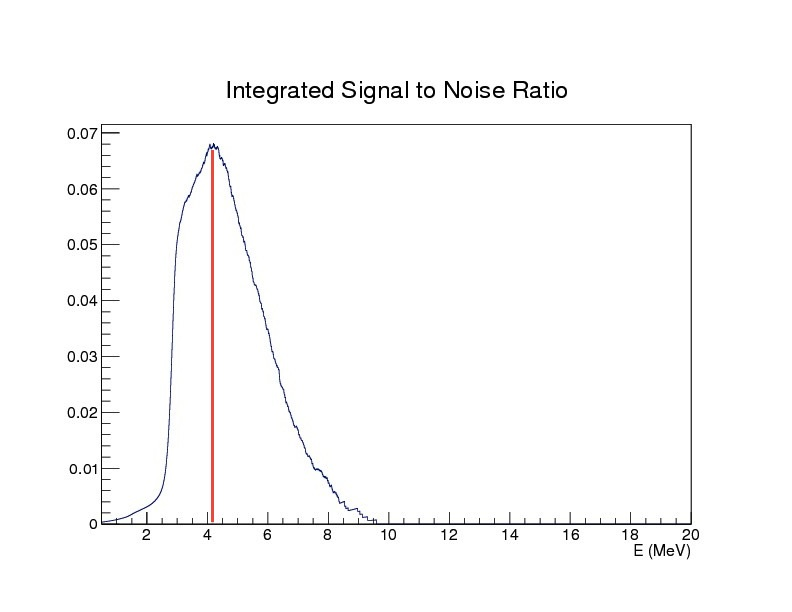
\includegraphics[width=\textwidth]{Paraphotons/Paraphoton_Signal_Noise_w_Cut.jpg}
\label{S/N}
\end{figure}

This region has the additional benefit of being well-described by a decaying exponential, allowing for model-based background subtraction. Being able to use a model-based subtraction, as opposed to a scaled rate subtraction, is very helpful for reducing the contribution caused by statistical error. Since the Off/Off data period has approximately 5 days of livetime while the On/On data has 156 days of livetime, being able to subtract a model of the background allows us to consider only the statistical error associated with the On/On  data, rather than having to scale up the Monte Carlo data sample or the Off/Off data. Fig. \ref{ROI Fit} shows a fit of a decaying exponential to the region of interest in the Off/Off data. We can scale this fit with livetime to the On/On data, allowing for a clean background subtraction.

\begin{figure}
\caption{Scalable fit to Off/Off data in the region of interest. This is the fit that is scaled with the On/On data as a background to be subtracted.}
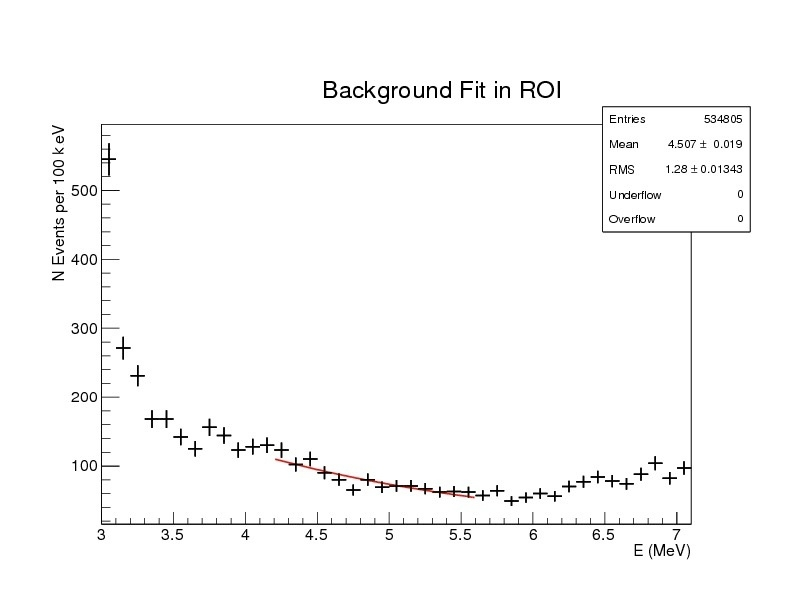
\includegraphics[width=\textwidth]{Paraphotons/Off_Off_Expo_edit.jpg}
\label{ROI Fit}
\end{figure}

\subsection{Sensitivity}
With our cuts established and region of interest characterized, we can then proceed to calculate the expected sensitivity of the experiment. We begin by determining the sources of error expected in the experiment. The first and most prominent source of error is the error associated with the cuts used to isolate the paraphotons. We determined this error by breaking the paraphoton Monte Carlo into sets of 5000 events and applying the cuts to each set. We then computed the standard deviation of the number of events left after all the cuts had been applied, giving the associated error. 

Another source of uncertainty is the reactor power. Thankfully, the reactor power error has been characterized as part of the Double Chooz search for neutrino signals, and we can make use of their determination of reactor power error, $5\%$ \cite{ReactorPaper}. The final source of experimental error is the livetime calculation. Livetime is calculated by subtracting the time lost to muon cuts from the total time. The error in this term comes from the calculation of total time, which is handled by counting the number of fixed rate triggers within each run. These triggers occur once per millisecond. However, they are not synchronized to the starts and ends of runs, resulting in a maximal error of 2 ms per one-hour run. Since all the errors above are uncorrelated, we add them in quadrature, giving $\sigma_{sys}^2 = \sigma_{Livetime}^2 + \sigma_{Power}^2 + \sigma_{Cuts}^2$.

A further source of error is the statistical error of the data sample. This is described by a Poisson distribution, which can be approximated as a Gaussian as there are many more than 3000 events contained in the region of interest, resulting in an expected statistical error of $ \sqrt{N} $ where $N$ is the number of events within the region of interest. Error on our background model was obtained by taking the error on our fit and evaluating the change in the number of events in the background model as a result of 1 $\sigma$ of change in our background parameters. 

We then perform a rate-based analysis, using the fit results to the Off/Off data as our background, and the paraphoton Monte Carlo as the signal. We used the Rolke  \cite{Rolke} fitter, developed in 2011. It makes use of a profile likelihood to generate confidence intervals in the presence of nuisance parameters.   These profile likelihoods have the benefit of providing a fully frequentist approach to sensitivity determination. Following the work of the SPring-8 paraphoton study, we determined 95$\%$ confidence intervals for our paraphoton search. These limits, as a function of livetime, can be seen in Fig. \ref{Sensitivity}.


 \begin{figure}
\caption{Expected sensitivity of Far-Detector-only data at 95\% confidence. $Y$-axis is $\chi$, the paraphoton mixing parameter, while $X$-axis is paraphoton mass.}
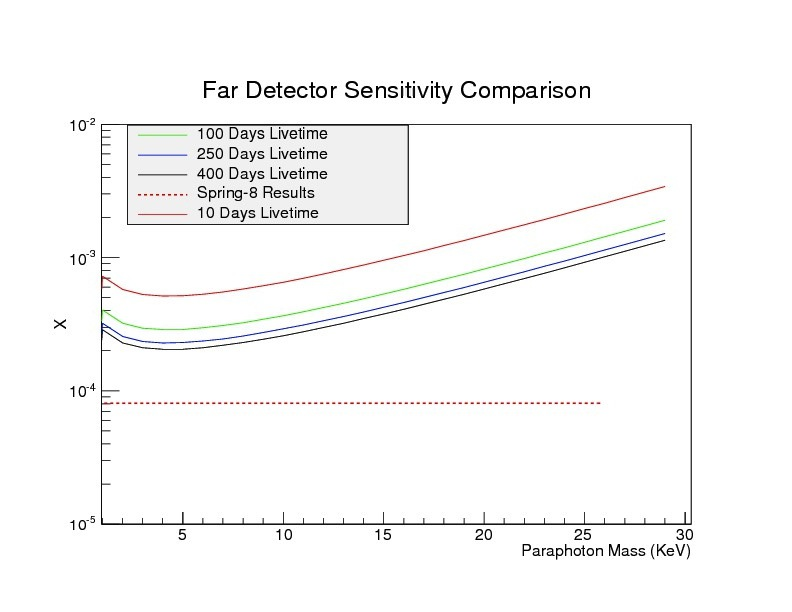
\includegraphics[width=\textwidth]{Paraphotons/FD_Sensitivity_Comparison.jpg}
\label{Sensitivity}
\end{figure}

 

\subsection{Paraphoton Injected Sample}
In order to validate our paraphoton search technique, we injected a sample of paraphotons into the Off/Off data. We then attempted to find the paraphoton signal within the paraphoton injected data and within the standard Off/Off data. Doing this comparison alerts us to the possibility of ``false positive" results, as well as acting as a practice run for the final fit. We injected paraphotons corresponding to a mixing parameter of $\chi = 10^{-2}$ and livetime equal to that of the Off/Off data. We chose a very large mixing parameter in order to ensure that the signal would be seen in the small amount of Off/Off livetime available. Fig. \ref{Injected Sample} shows the Off/Off spectrum along with the injected Off/Off spectrum and the paraphoton signal used for injection.  

\begin{figure}
\caption{Paraphoton-injected spectrum compared with the paraphoton spectrum and clean Off/Off spectrum used to generate it.}
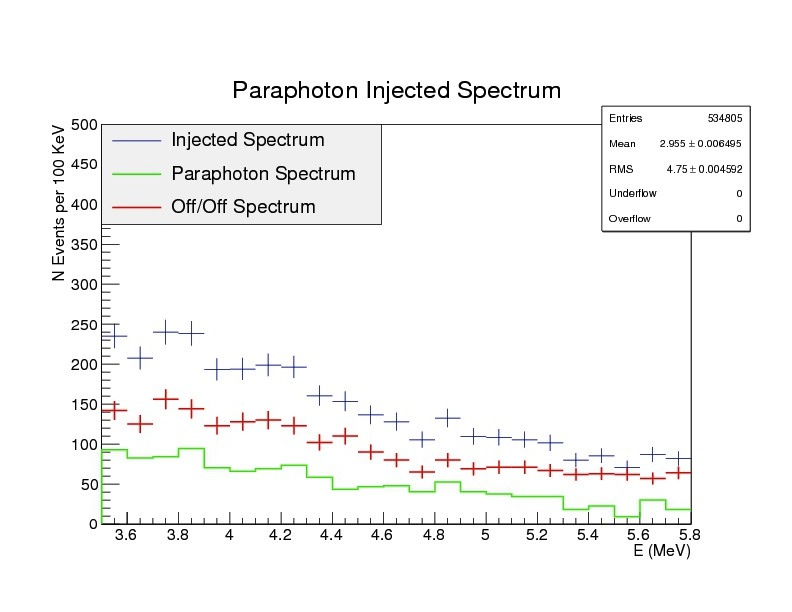
\includegraphics[width =\textwidth]{Paraphotons/Paraphoton_Injected_Spec.jpg}
\label{Injected Sample}
\end{figure}



We found a best fit rate of 550 events  $\pm$ 148 events over 5.29 days of livetime. The actual number of paraphoton events injected was 414 events, meaning that the fitting procedure functions as expected, returning a best fit result that was consistent with the true rate. 


\subsection{On/On and Final Fits}
The On/On data is processed in a similar fashion to the Off/Off data with the small exception that the files are too numerous to be processed in a single run, so the spectra and live-time are calculated by summing several processed files. The livetime of the On/On data sample is 156 days of livetime. After the On/On data is processed, we follow the same analysis procedure that we followed for the Off/Off injected sample. 

We begin by taking the Off/Off fit, and scaling it with livetime to the On/On data. Using that fit as the background, we then calculate best fit rate for paraphotons, as well as the lower limit on the rate given a 95\% confidence interval. In the event that the lower limit is less than or equal to zero, we calculate the critical rate, the rate at which the lower limit of the best fit rate is greater than zero. We then calculate the required mixing parameter, $\chi$, for each paraphoton mass tested  that would result in a detected rate equal to the critical rate. This mixing parameter is then used to set a limit for the maximal mixing parameter at each paraphoton mass. We see no evidence of paraphotons in our analysis, and the results of the subsequent rate study can be seen in Fig. \ref{FinalFit}.

\begin{figure}
\caption{Paraphoton limit at 95\% CL for this analysis of the Double Chooz Far Detector, showing a new laboratory limit in the range 26 keV $<E <$ 30 keV. $Y$-axis is $\chi$, the paraphoton mixing parameter, while $X$-axis is paraphoton mass.}
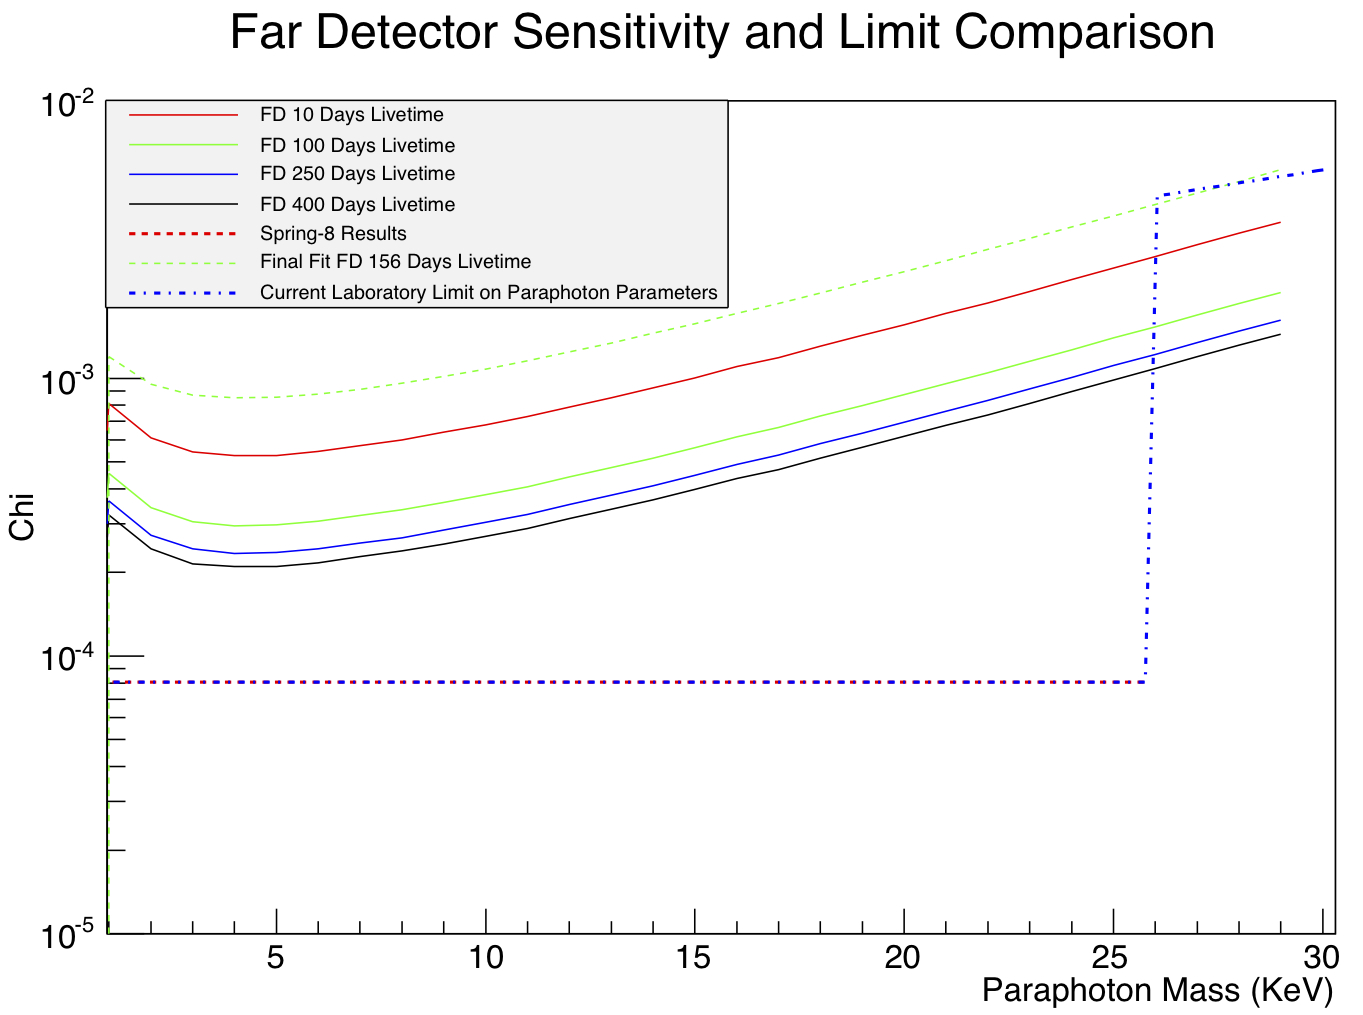
\includegraphics[width=\textwidth]{Paraphotons/Final_Fit_W_Sensitivity_156.jpg}
\label{FinalFit}
\end{figure}

We do not exceed the SPring-8 limits for the mass range of 1 KeV through 26 KeV. However, we do set new laboratory limits on the mixing parameter for paraphoton masses $26$ keV $< M_{para} < 30$keV. We did not exceed theoretical limits placed Rydberg transitions, but we broke new ground for laboratory paraphoton detection experiments \cite{Rydberg}. We obtained a minimal values of  $\chi > 4.23 \times 10^{-3}$ for $m_{para} =26$ keV paraphotons. 

\section{Future Work}
\label{sec:Future_Work}
The analysis shown above can be greatly improved through the introduction of the Double Chooz Near Detector. At 400 meters away from the reactor cores, the Near Detector is much closer than the Far Detector, meaning heavier paraphotons are less likely to decay during their flight and a larger total flux of paraphotons through the detector. With these improvements alone, our sensitivity improves to $\chi > 8.25 \times 10^{-5}$ for $m_{para} =2$ keV paraphotons after only 100 days of livetime, better than the SPring-8 limit. The combined results of these two improvements are shown graphically in Fig. \ref{FutureWork}. 

\begin{figure}
\caption{Expected Near Detector sensitivity compared with current limits, showing potential improvements. $Y$-axis is $\chi$, the paraphoton mixing parameter, while $X$-axis is paraphoton mass.}
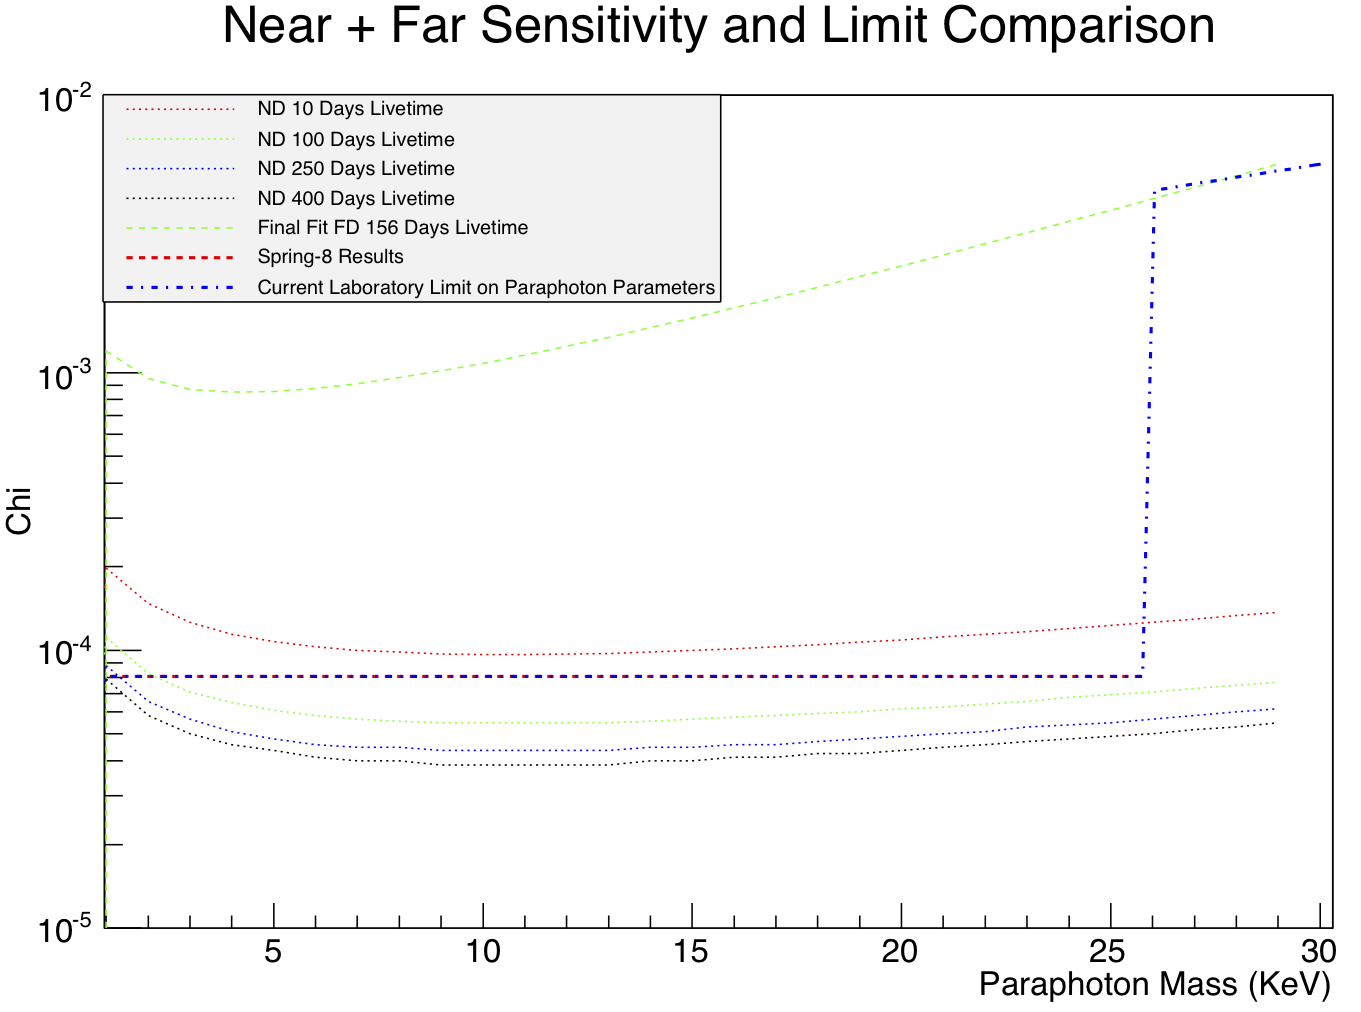
\includegraphics[width =\textwidth]{Paraphotons/Future_Fits_W_Limits_156.jpg}
\label{FutureWork}
\end{figure}

Additionally, there are expected upgrades to the front end electronics. These upgrades will allow for greatly improved pulse start time determination, potentially allowing for better use of the time likelihood to distinguish between paraphoton events and backgrounds. The effects of these upgrades are not shown in Fig. \ref{FutureWork}.  All of these improvements point towards greatly expanded sensitivity to detect or limit paraphotons in the Double Chooz experiment. 

\newpage

\section{Conclusion}
The thesis began with a discussion of the history of the neutrino and its role as catalyst for the development of new physics (Chap. \ref{chap:Intro}). Of particular importance is the discovery of neutrino oscillations and the resultant need for new, beyond the standard model physics. One of the experiments characterizing the frontiers of neutrino physics is Double Chooz, which was the focus of the second chapter. 

The subsequent chapter of the thesis (Chap. \ref{chap:Double Chooz}) discussed the Double Chooz experiment, a reactor-based search for the neutrino mixing angle $\theta_{13}$. We discussed the experiment in detail, including its primary mission, the measurement of $\theta_{13}$. We discussed the need for powerful calibration tools to allow for a precision measurement, particularly once the Near Detector phase of the experiment beings. 

The next chapter of the thesis (Chap. \ref{chap:AA}) details the design, development and use of a novel calibration system for the Double Chooz experiment, an Articulated Arm. The Articulated Arm is capable of making radioactive source deployments throughout the volume of the Neutrino Target, with a precision of $<$ 1 cm. The Articulated Arm is a powerful asset, able to validate detector response through direct comparison of on-axis and off-axis points. 
 
 The final chapter of the thesis (Chap. \ref{chap:Paraphotons}) detailed a search for paraphoton signals in the Double Chooz 3rd publication dataset. The paraphoton is a light, electrically neutral, axion-like particle, generated from adding a new $U(1)$ symmetry of baryon number - lepton Number. We searched for decays of these particles inside the Double Chooz Far Detector using a rate-based method, heavily leveraging the two-reactor-off period to allow for background calibration. We observed no events in excess of background, giving a new laboratory limit on the photon-paraphoton mixing angle $\chi$ at the 95$\%$ confidence level for paraphoton masses between 26 and 30kKeV, with a limiting value of $\chi > 4.23 \times 10^{-3}$ for $m_{para} =26$ keV paraphotons. We then discussed the future of the search for paraphotons in the Double Chooz experiment, particularly the benefits to the search that will occur when the Near Detector becomes operational, such as an improved sensitivity at the level of $\chi > 8.25 \times 10^{-5}$ for $m_{para} =2$ keV paraphotons after only 100 days of livetime. 

